\section{Uma avaliação do OpenFlow}

\begin{frame}{Uma avaliação do OpenFlow}

    \begin{itemize}
        \item Avaliar o protocolo OpenFlow através de um sistema de
            balanceamento de carga.
        \item Através dos recursos fornecidos pelo protocolo é possível 
            maximizar a justiça no balanceamento de carga em um serviço HTTP.
    \end{itemize}

    \begin{figure}[!htb]
        \centering
        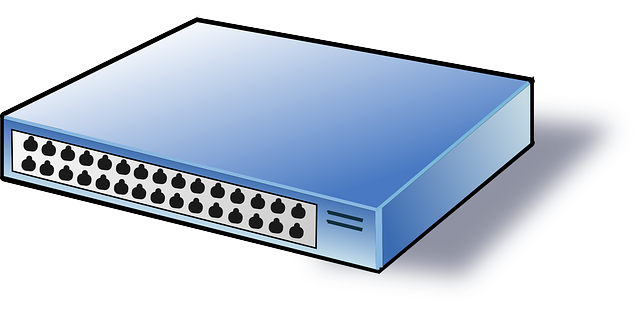
\includegraphics[scale=.3]{images/cartoon-switch}
    \end{figure}
\end{frame}


\begin{frame}{Contexto da avaliação}
    \begin{itemize}
        \setlength{\itemsep}{.5cm}
        \item Sistemas de balanceamento de carga são baseados em políticas 
            de balanceamento.
        \item Os serviços modernos devem ser escaláveis para atender a 
            milhões ou milhares de clientes.
        \item Os serviços devem ser distribuídos em vários servidores. 
        \item O OpenFlow permite políticas que podem se adaptar à aplicação 
            ou serviço.
    \end{itemize} 
\end{frame}


\begin{frame}{Projeto de implementação}

    \begin{itemize}
        \setlength{\itemsep}{.5cm}
        \item A solução resume-se em um balanceador de carga TCP.
        \item Um IP lógico é atribuído ao serviço
        \item Políticas de balanceamento decidem quais servidores serão
            escalonados
    \end{itemize}

\end{frame}

\begin{frame}{Fluxo de execução}

    \begin{figure}[htb!]
        \centering
        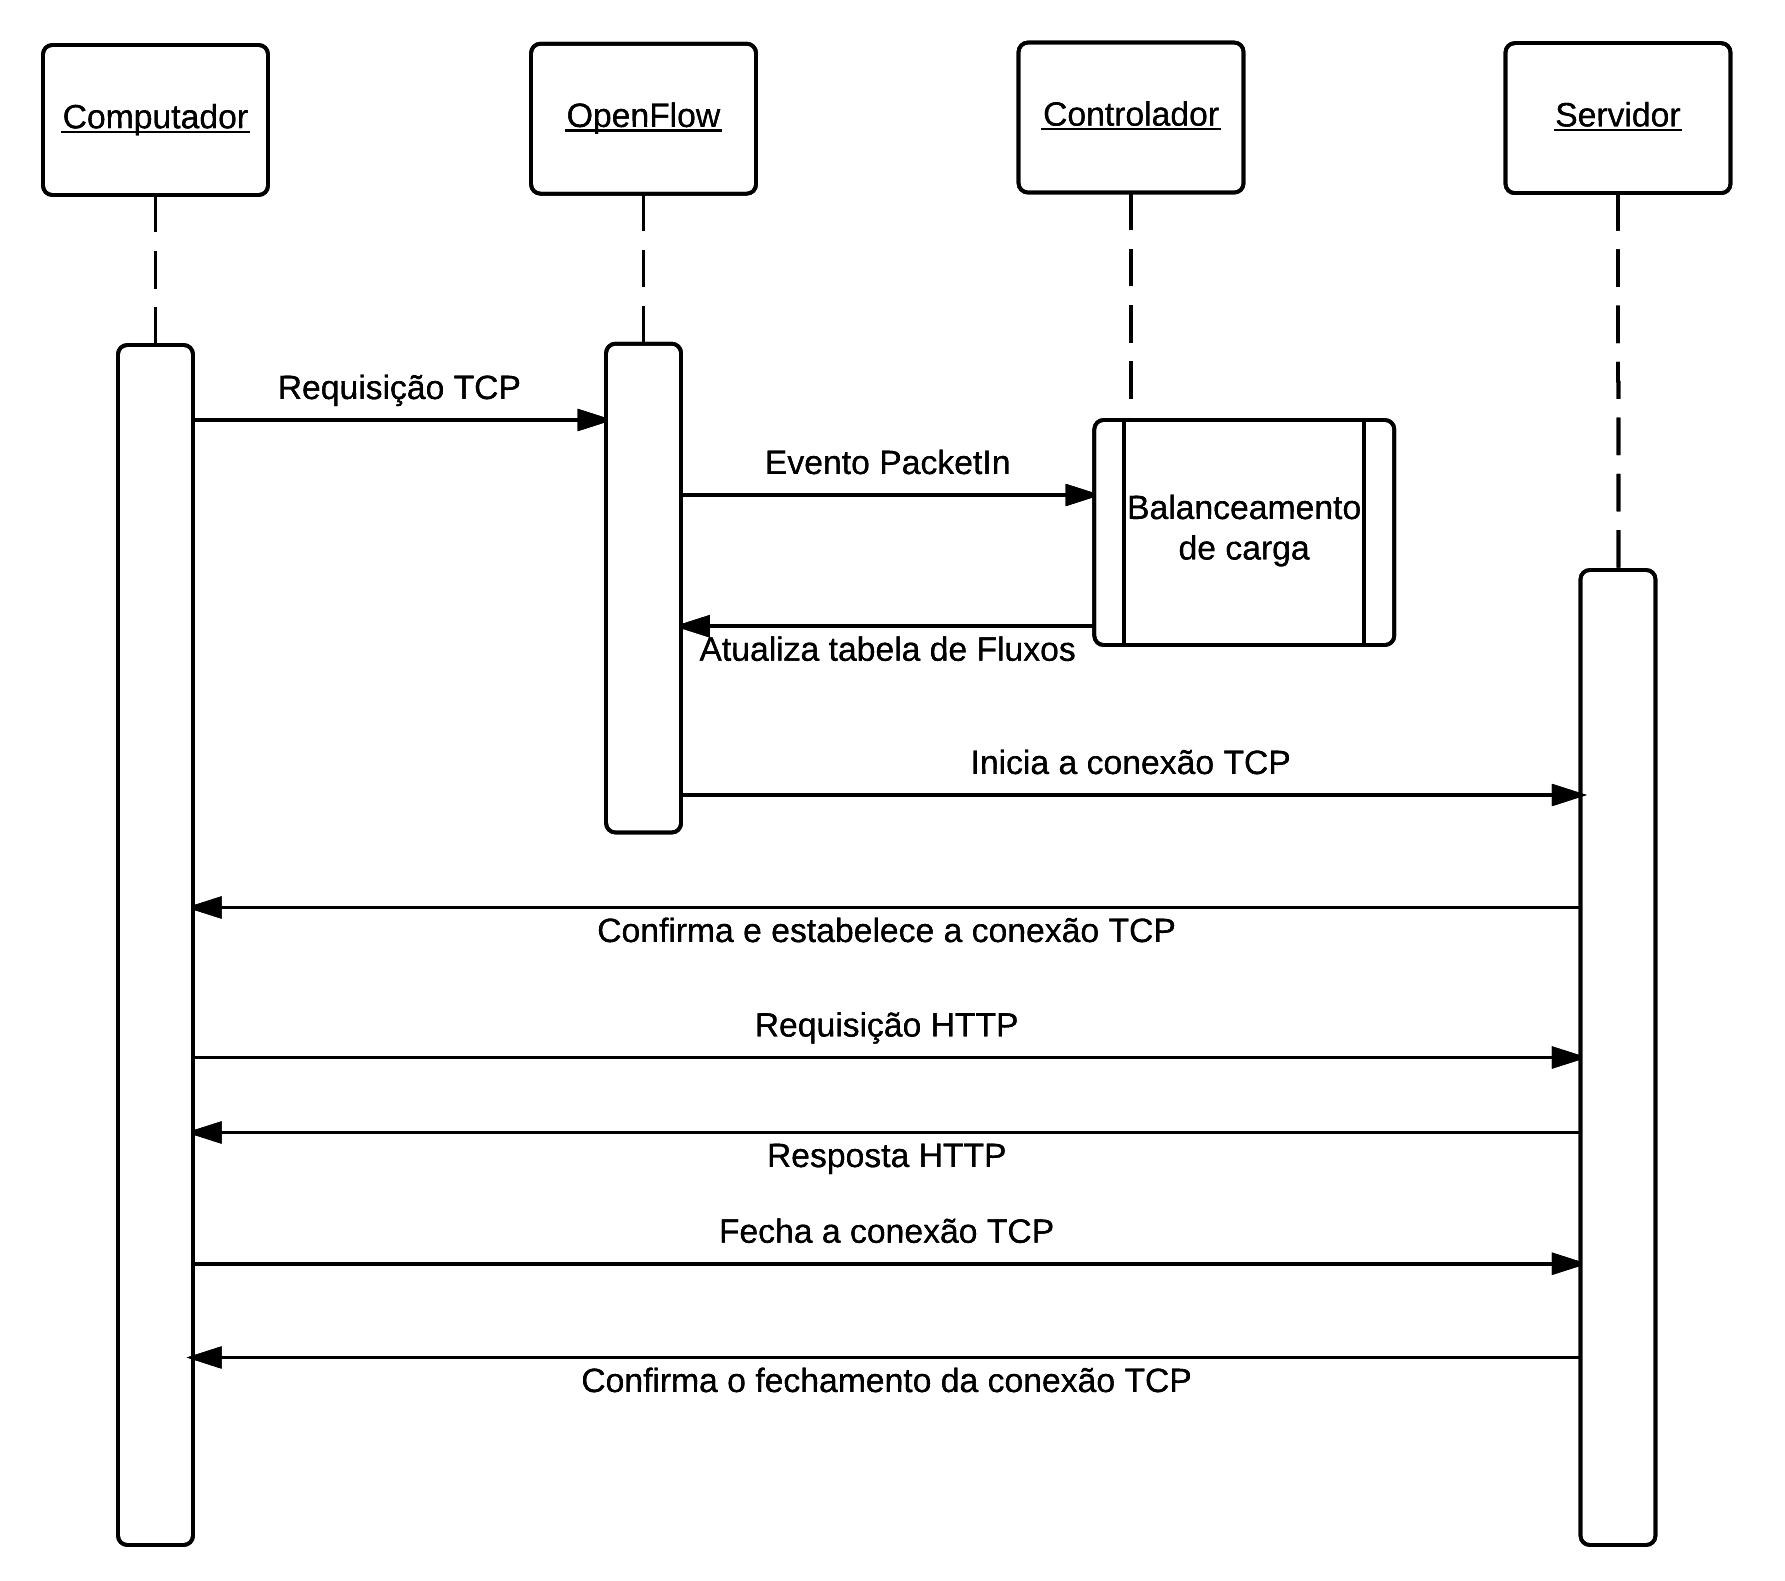
\includegraphics[scale=.55]{images/balancer-workflow}
    \end{figure}
\end{frame}


\begin{frame}{Políticas de balanceamento}
    
    \begin{enumerate}
        \setlength{\itemsep}{.5cm}
        \item Round-robin
        \item Aleatória
        \item Carga
        \item Fila 
        \item Mistura
    \end{enumerate}
\end{frame}

\begin{frame}{Ambiente dos experimentos}

    \begin{figure}[htb!]
        \centering
        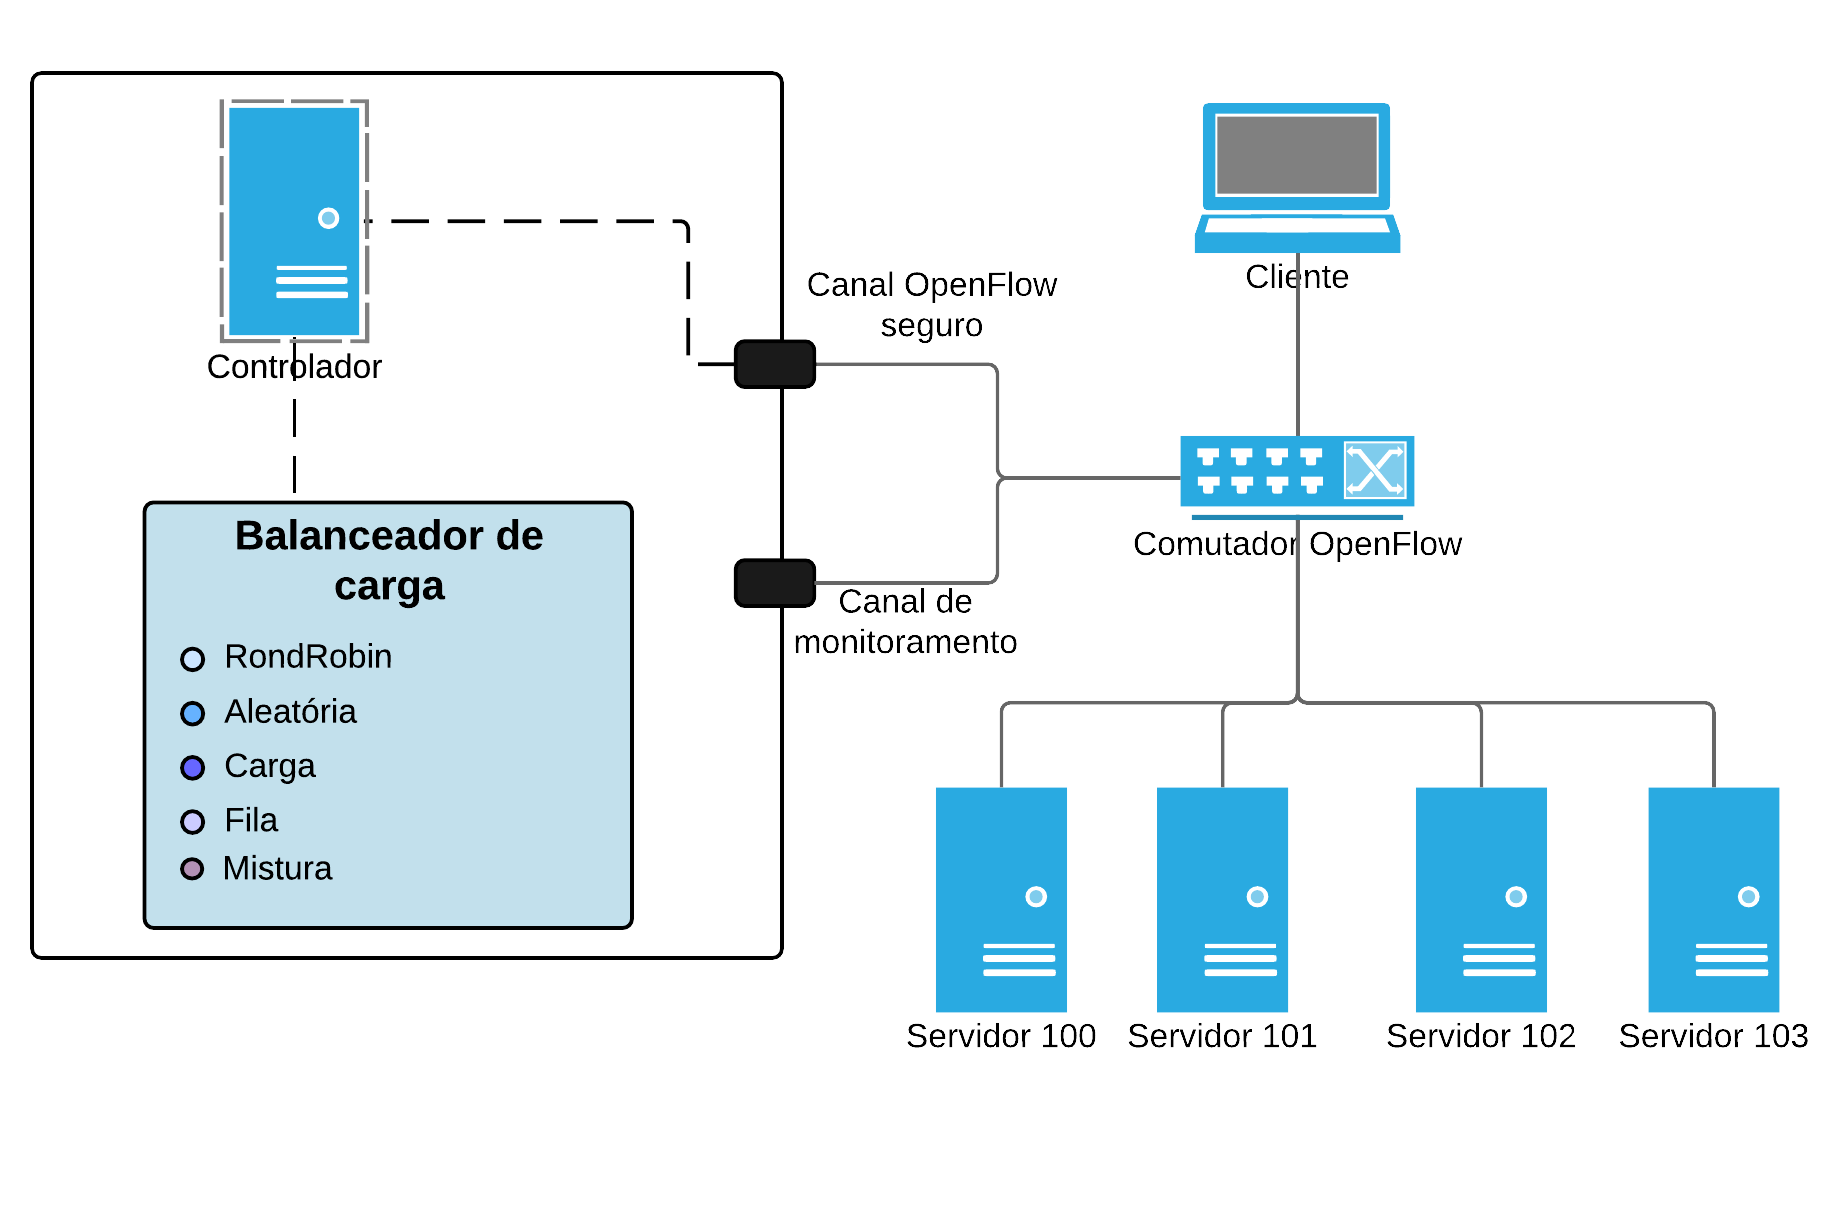
\includegraphics[scale=.7]{images/balancer-testbed-img}
    \end{figure}

\end{frame}


\begin{frame}{Distribuição de carga}

    \begin{figure}[htb!]
        \centering
        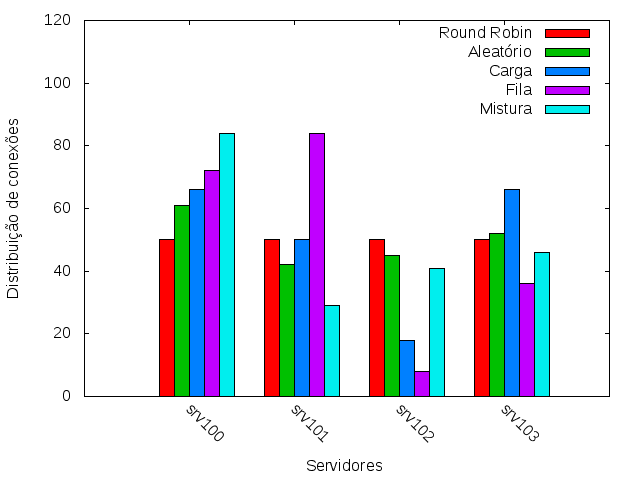
\includegraphics[scale=0.5]{images/balancer-distribution.png}
    \end{figure}

\end{frame}


\begin{frame}{Justiça em relação a carga dos servidores}

    \begin{figure}[htb!]
        \centering
        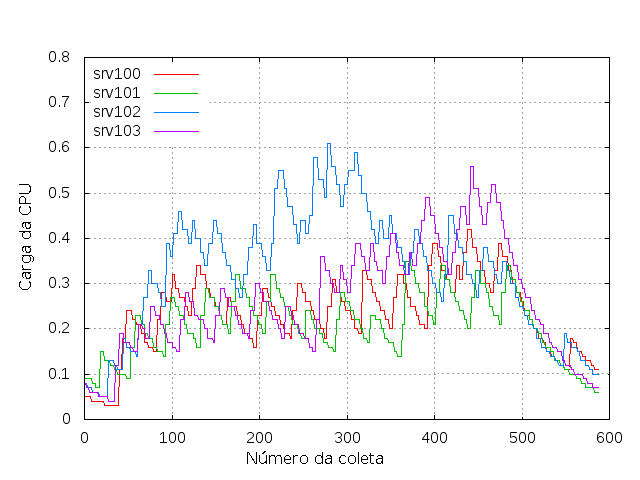
\includegraphics[scale=0.35]{images/balancer-serial-rr}
        \caption{RoundRobin em serial}
    \end{figure}

\end{frame}

\begin{frame}{Justiça em relação a carga dos servidores}

    \begin{figure}[htb!]
        \centering
        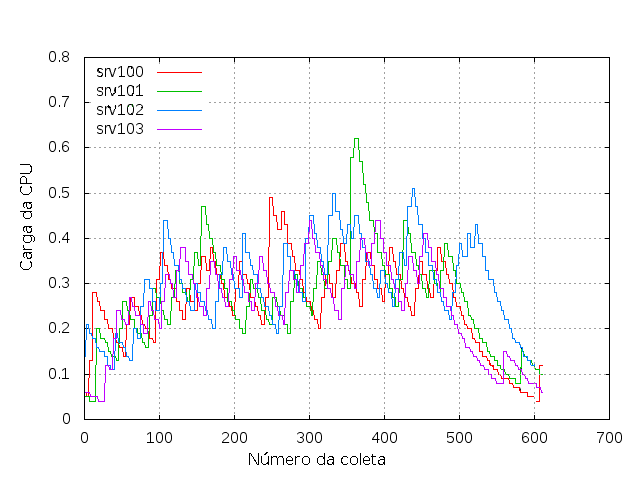
\includegraphics[scale=0.35]{images/balancer-serial-load}
        \caption{Carga em serial}
    \end{figure}

\end{frame}


\begin{frame}{Justiça em relação a carga dos servidores}
\begin{figure}[htb!]
    \centering
    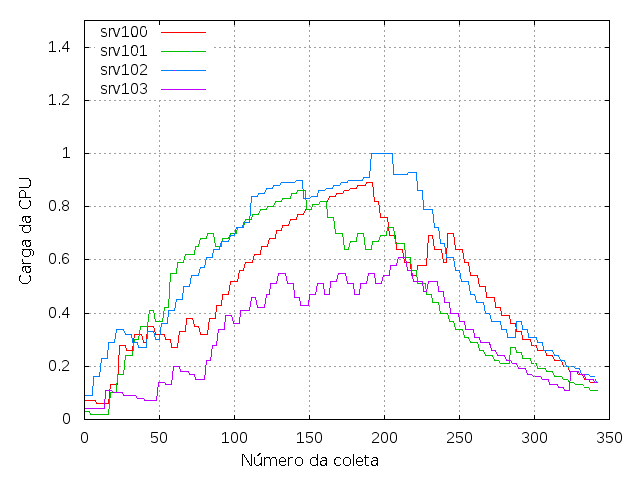
\includegraphics[scale=0.35]{images/balancer-parallel-rr}
    \caption{RoundRobin em paralelo}
\end{figure}
\end{frame}


\begin{frame}{Justiça em relação a carga dos servidores}
\begin{figure}[htb!]
    \centering
    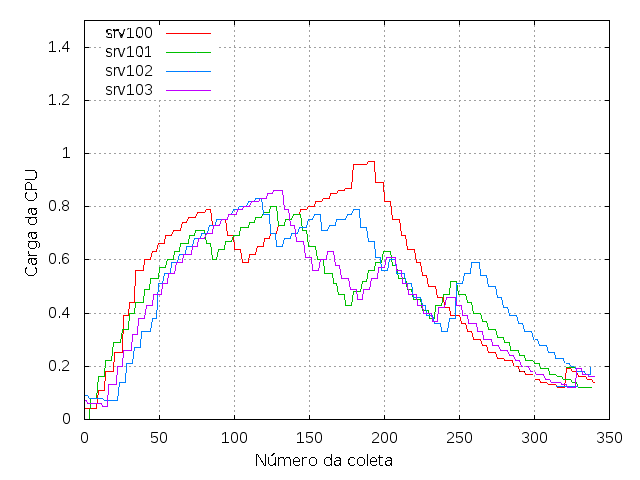
\includegraphics[scale=0.35]{images/balancer-parallel-load}
    \caption{Carga em paralelo}
\end{figure}

\end{frame}

\begin{frame}{Medição de justiça}
    \begin{itemize}
        \item Índice de justiça baseado na larguda de banda
            \footnote{A quantitative measure of fairness and discrimination for resource 
        allocation in shared computer system\citep{jain}}
    \end{itemize}
{\huge\centering
\[\jmath \left ( x_1, x_2,..., x_n \right ) = \frac{\left ( \sum_{i=1}^{n} x_i\right )^2}{n \cdot \sum_{i=1}^{n} x_i^2}\]
}

\end{frame}

\begin{frame}{Medição de justiça}

    \begin{figure}[htb!]
        \centering
        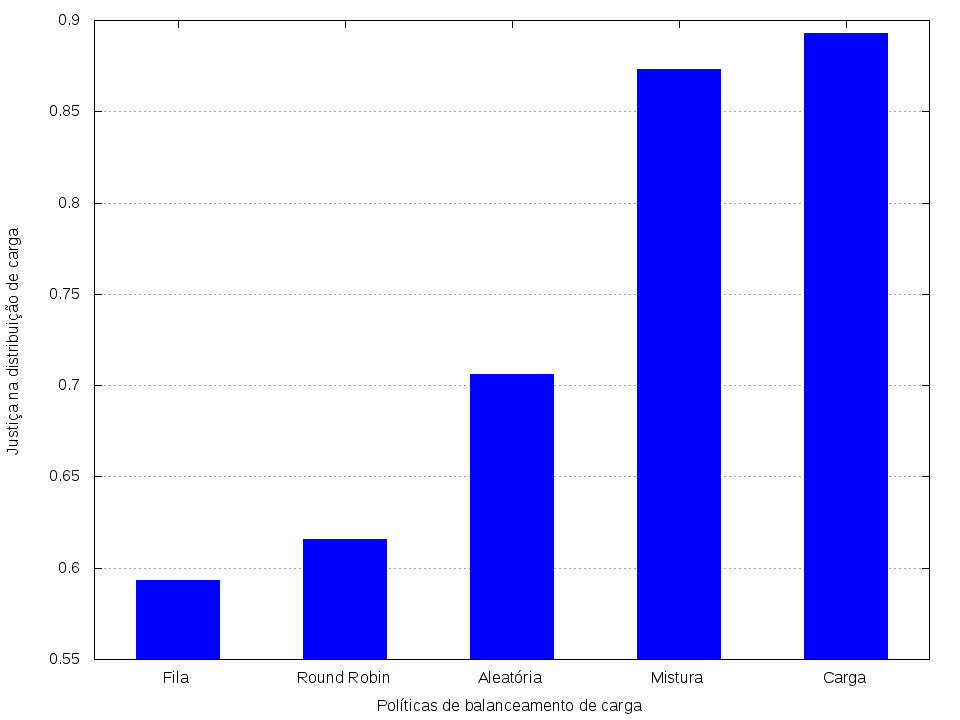
\includegraphics[scale=.35]{images/balancer-fairness}
    \end{figure}
\end{frame}


\begin{frame}{Largura de banda - TCP}

    \begin{figure}[htb!]
        \centering
        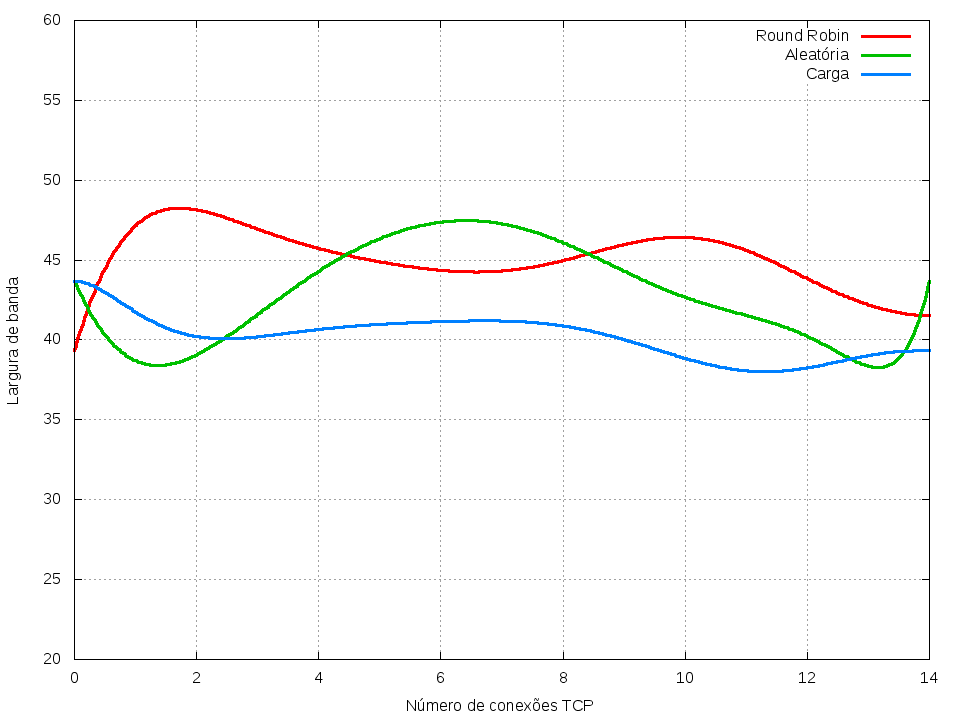
\includegraphics[scale=.35]{images/balancer-tcp-bandwidth}
    \end{figure}
\end{frame}


\begin{frame}{Tempo de resposta (latência) - HTTP}

    \begin{figure}[htb!]
        \centering
        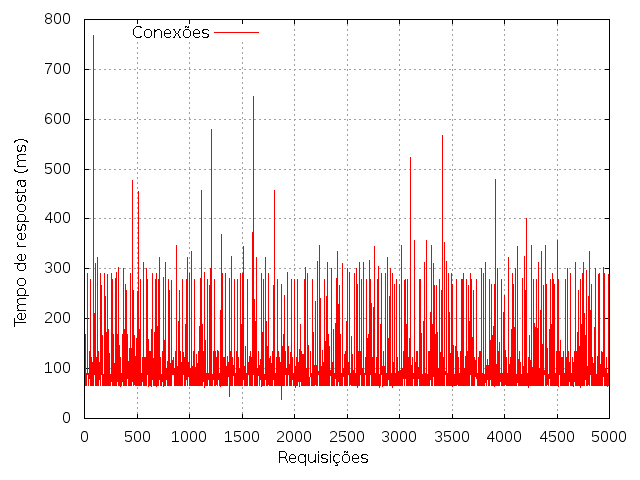
\includegraphics[scale=0.35]{images/balancer-http-full}
    \end{figure}
\end{frame}


\begin{frame}{Tempo de resposta (latência) - HTTP}

\begin{figure}[htb!]
    \centering
    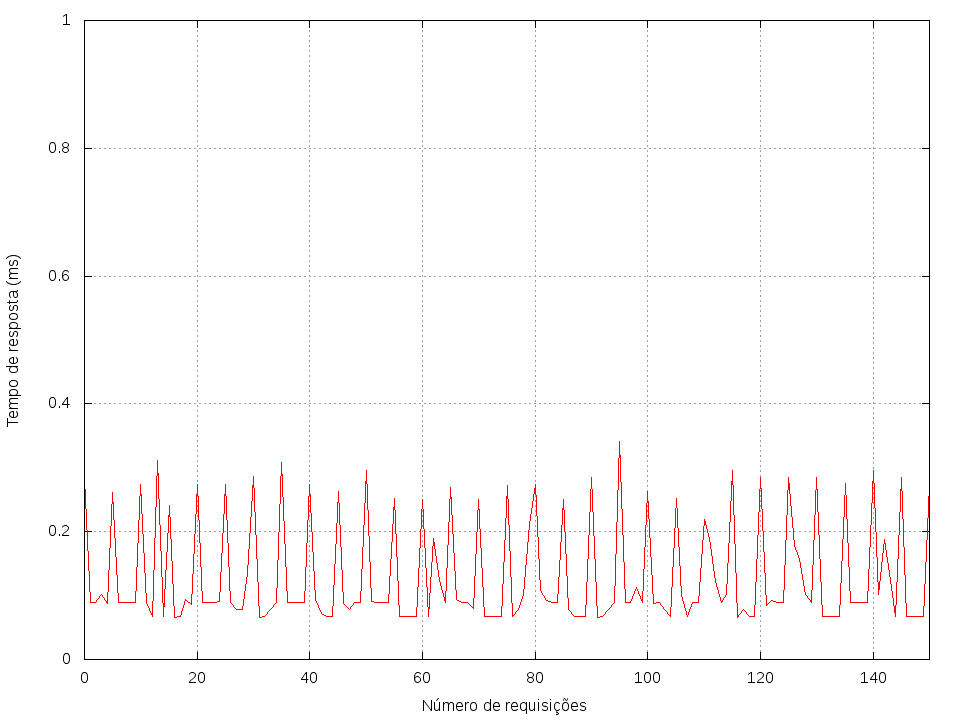
\includegraphics[scale=0.35]{images/balancer-http-zoom}
\end{figure}
\end{frame}

\begin{frame}{Tempo de resposta por política}
    \begin{figure}[htb!]
        \centering
        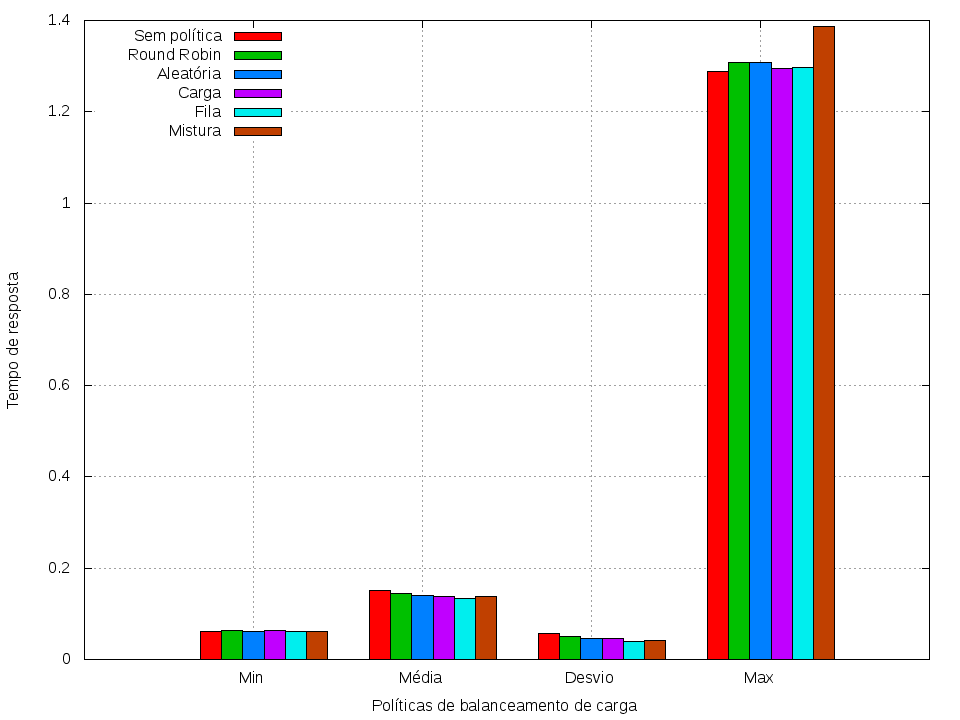
\includegraphics[scale=.35]{images/balancer-http-times}
    \end{figure}
\end{frame}

